\documentclass[11pt,xcolor=table,aspectratio=169]{beamer}
\usepackage{babel}
\usetheme{metropolis}
\usepackage{appendixnumberbeamer}
\usepackage{booktabs}

\title[Biomedical sensors 20/21]{Embedded measurement systems development}
\subtitle{Case studies}
\author{M. Pezzoli}
\date{A.Y. 2021-2022}
%\beamertemplatenavigationsymbolsempty
%\setbeamercovered{transparent} 
\usepackage{datetime2}
\usepackage{textpos}
\usepackage{pifont}
\usepackage{listings}
\newcommand{\cmark}{\ding{51}}%
\newcommand{\xmark}{\ding{55}}%


%Definizione colori
\definecolor{uniPVPink}{RGB}{157, 44, 73}
\definecolor{uniPVDarkBlue}{RGB}{14,12,24}
\definecolor{uniBGBlue}{RGB}{28,53,93}
\definecolor{paletteDarkGreen}{HTML}{4fa57a}
\definecolor{paletteLightGreen}{HTML}{9ee5b7}
\definecolor{uniBGLightBlue}{RGB}{148,177,223}
\definecolor{metropolisBackground}{RGB}{250,250,250}
\definecolor{orangeBeamer}{HTML}{FFD24A}

%Tikz
\usepackage{tikz}
\usetikzlibrary{automata,arrows.meta,shapes,calc,positioning,patterns,fit,3d,decorations.markings,matrix,spy,fadings,arrows}
\usepackage[americancurrents,arrowmos]{circuitikz}


\makeatletter
\tikzset{horizontal custom shading/.code={%
		\pgfmathsetmacro\tikz@vcs@middle{#1}
		\pgfmathsetmacro\tikz@vcs@bottom{\tikz@vcs@middle/2}
		\pgfmathsetmacro\tikz@vcs@top{(100-\tikz@vcs@middle)/2+\tikz@vcs@middle}
		\pgfdeclarehorizontalshading[tikz@axis@top,tikz@axis@middle,tikz@axis@bottom]{newaxis}{100bp}{%
			color(0bp)=(tikz@axis@bottom);
			color(\tikz@vcs@bottom bp)=(tikz@axis@bottom);
			color(\tikz@vcs@middle bp)=(tikz@axis@middle);
			color(\tikz@vcs@top bp)=(tikz@axis@top);
			color(100bp)=(tikz@axis@top)}
		\pgfkeysalso{/tikz/shading=newaxis}
	}
}
\makeatother  

\begin{tikzfadingfrompicture}[name=fade right]
	\shade[left color=transparent!5,middle color=transparent!5,
	right color=transparent!100] (0,0) rectangle (2,2);
\end{tikzfadingfrompicture}
%
\titlegraphic{
	\vspace{6cm}%
	\hspace{0.5cm}%
	
\includegraphics[height=1.4cm]{media/UniBG_logoComplete}
	\hspace{0.2cm}%
}

%\setbeamertemplate{frametitle}{%
%	\begin{beamercolorbox}{section in head/foot}
%		\vskip2pt\insertnavigation{\paperwidth}\vskip2pt
%	\end{beamercolorbox}%
%}
\tikzfading[name=fade right,left color=transparent!0,right color=transparent!100]
\setbeamertemplate{frametitle}{%
	\begin{tikzpicture}[remember picture,overlay]	
		%\fill[uniPVPink,path fading=fade right] (current page.north west) rectangle (\pagewidth, -.5cm);
		\fill[uniBGBlue!95](current page.north west) rectangle (\paperwidth ,-.5cm);
		\node[anchor=center] (logo) at (.89\paperwidth,0){
\includegraphics[height=.91cm,width=.91cm]{media/UniBG_logo}};
		\node[align=left,anchor=west](title) at (-.05\paperwidth,0){\insertframetitle};	
	\end{tikzpicture}%
\vskip15pt
}


% Numeri di pagina
\defbeamertemplate*{footline}{shadow theme}
{
	\leavevmode
	\hbox{\begin{beamercolorbox}[wd=.25\paperwidth,ht=2.1ex,dp=1.125ex,leftskip=.3cm plus1fil,rightskip=.3cm]{author in head/foot}%
			\usebeamerfont{author in head/foot}\insertframenumber\,/\,\inserttotalframenumber\hfill\insertshortauthor
		\end{beamercolorbox}
		\begin{beamercolorbox}[wd=.5\paperwidth,ht=2.1ex,dp=1.125ex,leftskip=.3cm,rightskip=.3cm plus1fil]{title in head/foot}
			\usebeamerfont{title in head/foot}\insertshorttitle
	\end{beamercolorbox}}
	\vskip0pt
}

\setbeamercolor*{palette primary}{use=structure,fg=white,bg=uniBGBlue}
\setbeamercolor{frametitle}{fg=white,bg=uniBGBlue}
\setbeamercolor{title separator}{bg=white,fg=uniBGBlue}
\setbeamercolor{structure}{fg=uniBGBlue,bg=white}
\setbeamercolor{alerted text}{fg=uniBGBlue}
\setbeamercolor{block title}{fg=uniBGBlue,bg=uniBGBlue!15}
% Figure
\usepackage{graphicx}
\usepackage{epstopdf}
\DeclareGraphicsExtensions{.eps,.png,.jpg,.pdf}
\usepackage{float}

\usepackage{makecell}



% Pacchetti matematica
\usepackage{amsmath}
\usepackage{amsthm}
\usepackage{amssymb}
\usepackage{mathtools}



\tikzset{
	set arrow inside/.code={\pgfqkeys{/tikz/arrow inside}{#1}},
	set arrow inside={end/.initial=>, opt/.initial=},
	/pgf/decoration/Mark/.style={
		mark/.expanded=at position #1 with
		{
			\noexpand\arrow[\pgfkeysvalueof{/tikz/arrow inside/opt}]{\pgfkeysvalueof{/tikz/arrow inside/end}}
		}
	},
	arrow inside/.style 2 args={
		set arrow inside={#1},
		postaction={
			decorate,decoration={
				markings,Mark/.list={#2}
			}
		}
	},
}

\definecolor{plotColor1}{RGB}{55,126,184}
\definecolor{plotColor2}{RGB}{228,26,28}
\definecolor{plotColor3}{RGB}{255,127,0}
\definecolor{plotColor4}{RGB}{152,78,163}
\definecolor{plotColor5}{RGB}{77,174,74}
\definecolor{plotColor6}{RGB}{255,255,51}
\definecolor{plotColor7}{RGB}{166,86,40}
\definecolor{plotColor8}{RGB}{247,129,191}
\definecolor{plotColor9}{RGB}{153,153,153}



\definecolor{grad1}{HTML}{FF0000}
\definecolor{grad2}{HTML}{FF5700}
\definecolor{grad3}{HTML}{FEAD00}
\definecolor{grad4}{HTML}{F9FE00}
\definecolor{grad5}{HTML}{A2FE00}
\definecolor{grad6}{HTML}{00FB0D}
\definecolor{grad7}{HTML}{00FD61}
\definecolor{grad8}{HTML}{00FCB6}
\definecolor{grad9}{HTML}{00ECFC}
\definecolor{grad10}{HTML}{0096FC}
\definecolor{grad11}{HTML}{0041FB}
\definecolor{grad12}{HTML}{1500FB}

%\definecolor{plotColor1}{RGB}{166,206,227}
%\definecolor{plotColor2}{RGB}{31,120,180}
%\definecolor{plotColor3}{RGB}{178,223,138}
%\definecolor{plotColor4}{RGB}{51,160,44}
%\definecolor{plotColor5}{RGB}{251,154,153}
%\definecolor{plotColor6}{RGB}{227,26,28}
%\definecolor{plotColor7}{RGB}{253,191,111}
%\definecolor{plotColor8}{RGB}{255,127,0}
%\definecolor{plotColor9}{RGB}{202,178,214}
%\definecolor{plotColor10}{RGB}{106,61,154}
%\definecolor{plotColor11}{RGB}{255,255,153}
%\definecolor{plotColor12}{RGB}{177,89,40}
%\definecolor{plotColor13}{RGB}{}
%\definecolor{plotColor14}{RGB}{}
%\definecolor{plotColor15}{RGB}{}
%\definecolor{plotColor16}{RGB}{}
%\definecolor{plotColor17}{RGB}{}
%\definecolor{plotColor18}{RGB}{}

%Pgrplots
\usepackage{pgfplots}
\usepackage[binary-units=true]{siunitx}
%\pgfplotsset{compat=newest}
\usepgfplotslibrary{units,groupplots,fillbetween}
\pgfplotscreateplotcyclelist{myColorList}{
	{plotColor1},
	{plotColor2},
	{plotColor3},
	{plotColor4},
	{plotColor5},
	{plotColor6},
	{plotColor7},
	{plotColor8},
	{plotColor9},
}

\pgfplotscreateplotcyclelist{slines}{
	{thin,solid},
	{thin,densely dashed},
	{thick,densely dotted},
	{thick,solid},
	{very thick,densely dashed},
	{very thick,densely dashdotdotted},
}
\pgfplotsset{
	every mark/.append style={fill={}},
	% Cycle list styles ----------------------------------------
	style colors/.style={cycle list name=myColorList},
	style lines/.style={cycle multiindex* list={myColorList\nextlist slines}},
	style marks/.style={cycle multiindex* list={myColorList\nextlist mark list*}},
	% Graph styles ---------------------------------------------
	graph/.style={grid=both,style #1},
	graph/.default={lines},
}


\usepackage{pgfplotstable}
%per ridimensionare le picture
\usepackage{adjustbox}
\usepackage{eurosym}

\DeclareSIUnit{\pers}{pers}
\DeclareSIUnit{\EUR}{\text{\euro}}
\sisetup{
	per-mode = fraction,
	inter-unit-product = \ensuremath{{}\cdot{}},
}
\usepackage{filecontents}





%BEGIN_FOLD Custom tikz shapes
%BEGIN_FOLD Custom PMOS
\pgfdeclareshape{customPMOS}{
	\anchor{center}{\pgfpointorigin}
	\anchor{text}{\pgfpoint{-.5\wd\pgfnodeparttextbox}{-.5\ht\pgfnodeparttextbox}}
	\savedanchor\mosS{\pgfpoint{.293cm}{.193cm}} % Source
	\anchor{S}{\mosS}
	\savedanchor\mosD{\pgfpoint{.293cm}{-.193cm}} % Drain
	\anchor{D}{\mosD}
	\savedanchor\mosG{\pgfpoint{-.45cm}{0}} % Gate
	\anchor{G}{\mosG}
	\savedanchor\mosB{\pgfpoint{0}{0}} % Bulk
	\anchor{B}{\mosB}
	\foregroundpath
	{ 
		\pgfsetlinewidth{0.014cm}\pgfpathmoveto{\pgfpoint{-.45cm}{0}}\pgfpathlineto{\pgfpoint{-.13cm}{0}}\pgfusepath{stroke}
		\pgfsetlinewidth{0.014cm}\pgfpathcircle{\pgfpoint{-.13cm}{0}}{.04cm}\pgfsetfillcolor{white}\pgfusepath{fill,stroke}
		\pgfsetlinewidth{0.05cm}\pgfpathmoveto{\pgfpoint{-.065cm}{.22cm}}\pgfpathlineto{\pgfpoint{-.065cm}{-.22cm}}\pgfusepath{stroke}
		\pgfsetlinewidth{0.014cm}\pgfpathmoveto{\pgfpoint{.3cm}{.2cm}}\pgfsetarrowsend{Triangle[length=1.5pt,angle'=30]}\pgfpathlineto{\pgfpoint{0}{.2cm}}\pgfusepath{stroke}
		\pgfsetarrowsend{}
		\pgfpathmoveto{\pgfpoint{0}{.22cm}}\pgfpathlineto{\pgfpoint{0}{-.22cm}}\pgfpathmoveto{\pgfpoint{0}{-.2cm}}\pgfpathlineto{\pgfpoint{.3cm}{-.2cm}}\pgfusepath{stroke}
	}
}
%END_FOLD
%BEGIN_FOLD Custom NMOS
\pgfdeclareshape{customNMOS}{
	\anchor{center}{\pgfpointorigin}
	\anchor{text}{\pgfpoint{-.5\wd\pgfnodeparttextbox}{-.5\ht\pgfnodeparttextbox}}
	\savedanchor\mosS{\pgfpoint{.293cm}{.193cm}} % Drain
	\anchor{S}{\mosS}
	\savedanchor\mosD{\pgfpoint{.293cm}{-.193cm}} % Source
	\anchor{D}{\mosD}
	\savedanchor\mosG{\pgfpoint{-.45cm}{0}} % Gate
	\anchor{G}{\mosG}
	\savedanchor\mosB{\pgfpoint{0}{0}} % Bulk
	\anchor{B}{\mosB}
	\foregroundpath
	{ 
		\pgfsetlinewidth{0.014cm}\pgfpathmoveto{\pgfpoint{-.45cm}{0}}\pgfpathlineto{\pgfpoint{-.065cm}{0}}\pgfusepath{stroke}
		\pgfsetlinewidth{0.05cm}\pgfpathmoveto{\pgfpoint{-.065cm}{.22cm}}\pgfpathlineto{\pgfpoint{-.065cm}{-.22cm}}\pgfusepath{stroke}
		\pgfsetlinewidth{0.014cm}\pgfpathmoveto{\pgfpoint{0}{-.2cm}}\pgfsetarrowsend{Triangle[length=1.5pt,angle'=30]}\pgfpathlineto{\pgfpoint{.3}{-.2cm}}\pgfsetarrowsend{}\pgfusepath{stroke}
		\pgfpathmoveto{\pgfpoint{0}{-.22cm}}\pgfpathlineto{\pgfpoint{0}{.22cm}}\pgfpathmoveto{\pgfpoint{0}{.2cm}}\pgfpathlineto{\pgfpoint{.3cm}{.2cm}}\pgfusepath{stroke}
	}
}
%END_FOLD
%BEGIN_FOLD Custom controlled switch (negated logic)
\pgfdeclareshape{customVCSwitchN}{
	\anchor{center}{\pgfpointorigin}
	\anchor{text}{\pgfpoint{-.5\wd\pgfnodeparttextbox}{-.5\ht\pgfnodeparttextbox}}
	\savedanchor\sIN{\pgfpoint{-.35cm}{0}} % IN1
	\anchor{INA}{\sIN}
	\savedanchor\sOUT{\pgfpoint{.35cm}{0}} % IN2
	\anchor{INB}{\sOUT}
	\savedanchor\sCTRL{\pgfpoint{0}{.293cm}} % Control
	\anchor{CTRL}{\sCTRL}
	\foregroundpath
	{ 
		\pgfsetlinewidth{0.014cm}
		\pgfpathmoveto{\pgfpoint{.35cm}{0}}\pgfpathlineto{\pgfpoint{.12cm}{0}}\pgfpathlineto{\pgfpointpolar{150}{.14cm}}
		\pgfpathmoveto{\pgfpoint{-.12cm}{0}}\pgfpathlineto{\pgfpoint{-.35cm}{0}}
		\pgfpathrectanglecorners{\pgfpoint{-.2cm}{-.075cm}}{\pgfpoint{.2cm}{.15cm}}
		\pgfpathmoveto{\pgfpoint{0}{.23cm}}\pgfpathlineto{\pgfpoint{0}{.3cm}}
		\pgfusepath{stroke}
		
		\pgfsetlinewidth{0.015cm}
		\pgfpathcircle{\pgfpoint{0}{.19cm}}{.04cm}
		\pgfsetfillcolor{white}
		\pgfusepath{fill,stroke}
	}
}
%END_FOLD
%BEGIN_FOLD Custom external signal switch
\pgfdeclareshape{customExtVCSwitch}{
	\anchor{center}{\pgfpointorigin}
	\anchor{text}{\pgfpointdiff{\pgfpoint{.5\wd\pgfnodeparttextbox}{.5\ht\pgfnodeparttextbox}}{\pgfpoint{0}{.6cm}}}	
	\savedanchor\sIN{\pgfpoint{-.35cm}{0}} % IN1
	\anchor{INA}{\sIN}
	\savedanchor\sOUT{\pgfpoint{.35cm}{0}} % IN2
	\anchor{INB}{\sOUT}
	\savedanchor\sNAME{\pgfpointadd{\pgfpoint{-.5\wd\pgfnodeparttextbox}{-.5\ht\pgfnodeparttextbox}}{\pgfpoint{0}{.5cm}}} % Signal name
	\anchor{NAME}{\sNAME}
	
	\foregroundpath
	{ 
		\pgfsetlinewidth{0.015cm}
		\pgfpathmoveto{\pgfpoint{.35cm}{0}}\pgfpathlineto{\pgfpoint{.12cm}{0}}\pgfpathlineto{\pgfpointpolar{150}{.14cm}}
		\pgfpathmoveto{\pgfpoint{-.12cm}{0}}\pgfpathlineto{\pgfpoint{-.35cm}{0}}
		\pgfpathrectanglecorners{\pgfpoint{-.2cm}{-.075cm}}{\pgfpoint{.2cm}{.15cm}}
		\pgfpathmoveto{\pgfpoint{0}{.15cm}}\pgfpathlineto{\pgfpoint{0}{.3cm}}
		\pgfusepath{stroke}
		
		\pgfpathmoveto{\pgfpoint{0cm}{.28cm}}\pgfpathlineto{\pgfpoint{.05cm}{.35cm}}\pgfpathlineto{\pgfpoint{.05cm}{.45cm}}\pgfpathlineto{\pgfpoint{-.05cm}{.45cm}}\pgfpathlineto{\pgfpoint{-.05cm}{.35cm}}
		\pgfsetfillcolor{black}
		\pgfusepath{fill}
	}
}
%END_FOLD
%BEGIN_FOLD Custom external signal switch (negated logic)
\pgfdeclareshape{customExtVCSwitchN}{
	\anchor{center}{\pgfpointorigin}
	\anchor{text}{\pgfpointdiff{\pgfpoint{.5\wd\pgfnodeparttextbox}{.5\ht\pgfnodeparttextbox}}{\pgfpoint{0}{.6cm}}}
	\savedanchor\sIN{\pgfpoint{-.35cm}{0}} % IN1
	\anchor{INA}{\sIN}
	\savedanchor\sOUT{\pgfpoint{.35cm}{0}} % IN2
	\anchor{INB}{\sOUT}
	\savedanchor\sNAME{\pgfpointadd{\pgfpoint{-.5\wd\pgfnodeparttextbox}{-.5\ht\pgfnodeparttextbox}}{\pgfpoint{0}{.5cm}}} % Signal name
	\anchor{NAME}{\sNAME}
	
	\foregroundpath
	{ 
		\pgfsetlinewidth{0.015cm}
		\pgfpathmoveto{\pgfpoint{.35cm}{0}}\pgfpathlineto{\pgfpoint{.12cm}{0}}\pgfpathlineto{\pgfpointpolar{150}{.14cm}}
		\pgfpathmoveto{\pgfpoint{-.12cm}{0}}\pgfpathlineto{\pgfpoint{-.35cm}{0}}
		\pgfpathrectanglecorners{\pgfpoint{-.2cm}{-.075cm}}{\pgfpoint{.2cm}{.15cm}}
		\pgfpathmoveto{\pgfpoint{0}{.23cm}}\pgfpathlineto{\pgfpoint{0}{.3cm}}
		\pgfusepath{stroke}
		
		\pgfpathmoveto{\pgfpoint{0cm}{.28cm}}\pgfpathlineto{\pgfpoint{.05cm}{.35cm}}\pgfpathlineto{\pgfpoint{.05cm}{.45cm}}\pgfpathlineto{\pgfpoint{-.05cm}{.45cm}}\pgfpathlineto{\pgfpoint{-.05cm}{.35cm}}
		\pgfsetfillcolor{black}
		\pgfusepath{fill}
		
		\pgfsetlinewidth{0.015cm}
		\pgfpathcircle{\pgfpoint{0}{.19cm}}{.04cm}
		\pgfsetfillcolor{white}
		\pgfusepath{fill,stroke}
	}	
}
%END_FOLD
%BEGIN_FOLD Custom input
\pgfdeclareshape{customINSignal}{
	\anchor{center}{\pgfpointorigin}
	\anchor{text}{\pgfpointadd{\pgfpoint{-\wd\pgfnodeparttextbox}{-.5\ht\pgfnodeparttextbox}}{\pgfpoint{-.23cm}{0cm}}}
	\savedanchor\wire{\pgfpoint{-.1cm}{0}} % Wire
	\anchor{W}{\wire}
	\foregroundpath
	{ 
		\pgfpathmoveto{\pgfpoint{0cm}{0cm}}\pgfpathlineto{\pgfpoint{-.05cm}{.05cm}}\pgfpathlineto{\pgfpoint{-.20cm}{.05cm}}\pgfpathlineto{\pgfpoint{-.20cm}{-.05cm}}\pgfpathlineto{\pgfpoint{-.05cm}{-.05cm}}
		\pgfsetfillcolor{black}
		\pgfusepath{fill}
		
	}
}
%END_FOLD
%BEGIN_FOLD Custom output
\pgfdeclareshape{customOUTSignal}{
	\anchor{center}{\pgfpointorigin}
	\anchor{text}{\pgfpointadd{\pgfpoint{-.5\wd\pgfnodeparttextbox}{-.5\ht\pgfnodeparttextbox}}{\pgfpoint{-.23cm}{0cm}}}
	\savedanchor\wire{\pgfpoint{-.1cm}{0}} % Wire
	\anchor{W}{\wire}
	\foregroundpath
	{ 
		\pgfpathmoveto{\pgfpoint{0cm}{0cm}}\pgfpathlineto{\pgfpoint{0cm}{.05cm}}\pgfpathlineto{\pgfpoint{-.15cm}{.05cm}}\pgfpathlineto{\pgfpoint{-.20cm}{0cm}}\pgfpathlineto{\pgfpoint{-.15cm}{-.05cm}}\pgfpathlineto{\pgfpoint{0cm}{-.05cm}}
		\pgfsetfillcolor{black}
		\pgfusepath{fill}
		
	}
}
%END_FOLD

%BEGIN_FOLD Custom arrows
\tikzstyle{vecArrow} = [thick, decoration={markings,mark=at position1 with {\arrow[semithick]{open triangle 60}}},double distance=1.4pt, shorten >= 5.5pt,preaction = {decorate},postaction = {draw,line width=1.4pt, white,shorten >= 4.5pt}]
\tikzstyle{innerWhite} = [semithick, white,line width=1.4pt, shorten >= 4.5pt]
%END_FOLD

%END_FOLD

\definecolor{mDarkTeal}{HTML}{23373b}
\usepackage{appendixnumberbeamer}

\begin{document}
	
	\maketitle
	\begin{frame}
		\frametitle{Project phase}
		The first development phase aims to draft a project, starting from the specifications document:
			\begin{itemize}
				\item Specifications document is meant to concretize abstract requirements into concrete goals/limitations.
				\item Always try to minimize size, power consumption and cost if this does not hinder other requirements.
				\item Choose sensors, memory and comms according to specs, then choose microcontroller to fit.
				\item Choose battery and power management ICs after defining other system components to fit.	
			\end{itemize}
	\end{frame}
	
	\begin{frame}
		\frametitle{Case study 1 - Winter}
		\textbf{Request}: develop an inertial and environmental monitoring system.\\
		\textbf{Additional constraints}:
		\begin{itemize}
			\item must have wireless comm capabilities;
			\item long log sessions (raw) to be stored on-board;
			\item leave possibilities for future developments/additional sensors;
		\end{itemize}
	\end{frame}

	\begin{frame}
		\frametitle{Winter - Specification document}
		\only<1>{
			What should be in the specification document for Winter?
			\begin{itemize}
				\item Sensor choices: \begin{itemize}
					\item Must have: axl, gyro, temperature, humidity
					\item Maybe: magn, pressure
				\end{itemize}
				\item axl must reach 10g, gyro 1000dps full-scale
				\item BT seems the best solution for wireless
				\item long log sessions = memory requirements; 
				\item expose some peripherals for future developments.
			\end{itemize}
		}
		\only<2>{
			Refining specifications:
			\begin{itemize}
				\item axl: at least 10g FS, look for best performer afterwards;
				\item gyro: at least 1000dps FS, look for best performer afterwards;
				\item BT: use BLE, use module to have it already certified;
				\item Memory: SD for ease of use, \SI{521}{\mega\byte} would be plenty
				\item Other: log usually requires precise timekeeping, so add a LSE crystal
			\end{itemize}
		}
	\end{frame}

	\begin{frame}
		\frametitle{Winter - Accelerometer + gyro}
		\only<1>{
			Choices to make:
			\begin{itemize}
				\item Do we use two separated ICs for accelerometer and gyroscope?
				\item What peripheral will we aim to use?
				\item What characteristics do we keep an eye out for?
			\end{itemize}
		}
		\only<2>{
			Choices for Winter:
			\begin{itemize}
				\item Better to save space, the board will be already cramped
				\item SPI should be better to aim for faster transmission 
				\item Important features:\begin{itemize}
					\item Accelerometer and gyroscope full-scales
					\item Accelerometer ODR
					\item Gyroscope offset
					\item Gyroscope ODR
					\item power consumption and size
				\end{itemize}
			\end{itemize}
		}
		\only<3>{
			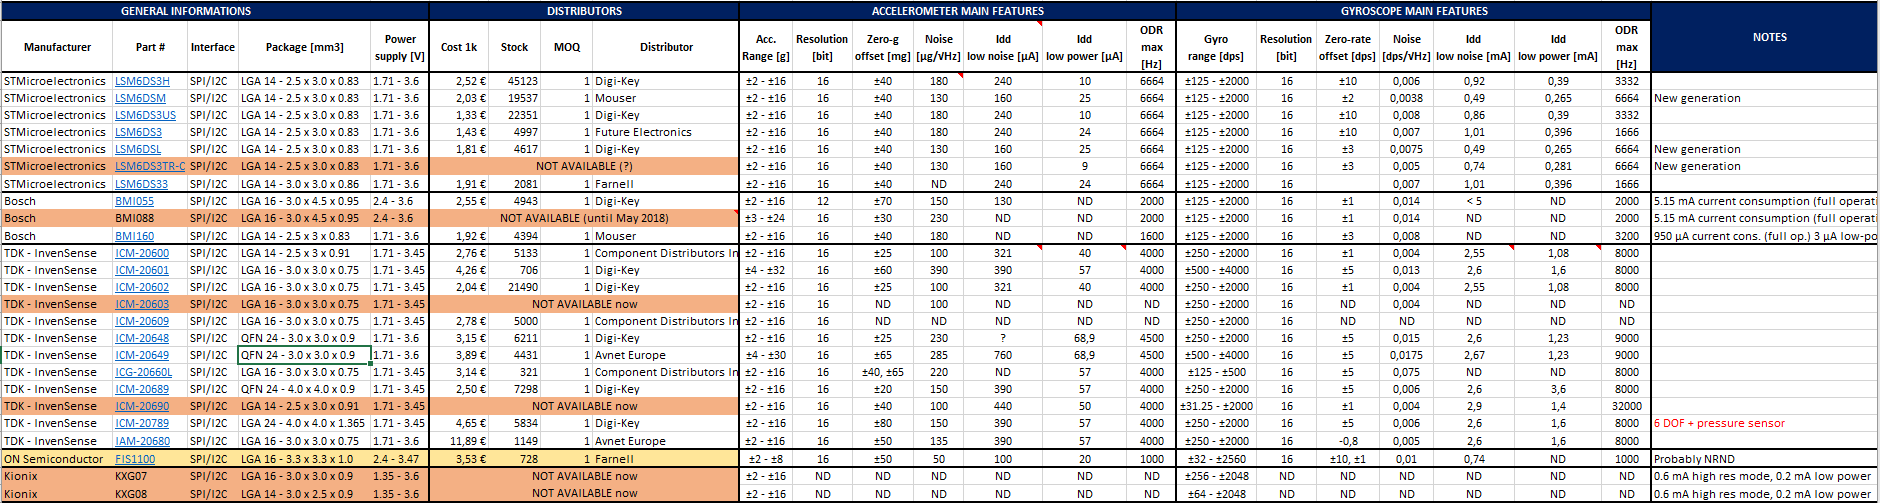
\includegraphics[width=\textwidth]{media/axl_xls.png}
		}
		\only<4>{
			The \textbf{LSM6DSL} was chosen. Important features:
			\begin{itemize}
				\item $\pm 2$g - $\pm 16$g selectable full-scale;
				\item \SI{6}{\kilo\hertz} ODR, highest among the ones considered
				\item \SI{16}{\bit} resolution, highest among the ones considered
				\item $\pm 3$ dps gyro offset, one of the lowest among the ones considered
				\item one of the lowest current consumptions among the ones considered
			\end{itemize}
		}
		
	\end{frame}

	\begin{frame}
		\frametitle{Winter - Temperature + humidity sensor}
		Humidity and temperature combo sensors are pretty widespread, so we can opt for those in order to save space. Specifications are not that strict since we need to measure ambient temperature (\SI{-20}{\degreeCelsius} to \SI{50}{\degreeCelsius}) and relative humidity (\SI{10}{\percent} to \SI{90}{\percent}). We ended up choosing the \textbf{HTS221} sensor.\\
		The main characteristics are:
		\begin{itemize}
			\item Same supply range as accelerometer;
			\item Humidity range \SI{0}{\percent} to \SI{100}{\percent};
			\item Temperature range \SI{-40}{\degreeCelsius} to \SI{120}{\degreeCelsius};
			\item \SI{0.5}{\degreeCelsius} accuracy in the indoor temperature range.
		\end{itemize}
	\end{frame}

	\begin{frame}
		\frametitle{Winter - Pressure sensor}
		Again, specifications are not that strict because we need to measure ambient pressure. We ended up choosing the \textbf{LPS22HH} sensor.\\
		The main characteristics are:
		\begin{itemize}
			\item \SI{260}{\hecto\pascal} to \SI{1260}{\hecto\pascal};
			\item \SI{4}{\micro\ampere} current consumption;
			\item Same supply range as accelerometer (and temp+hum sensors).
		\end{itemize}
	\end{frame}

	\begin{frame}
		\frametitle{Winter - Memory}
		We already chose the SD memory in the specification document, here we can confirm that the size of the SD card will fit our needs:
		\begin{itemize}
			\item \textbf{Case 1}: Inertial data log; let's say that we are in a worst case scenario and we want to log @\SI{100}{\hertz}.
			\item \textbf{Case 2}: Environmental log; let's say we want to log environmental data @\SI{1}{\hertz}.
		\end{itemize}
	\end{frame}

	\begin{frame}
		\frametitle{Winter - Communication}
		We already considered the BT as the best choice for the communication, and we are going to use a module to ease the development process and certification procedure. In the case of radio modules, it is often a choice of familiarity with a given module, since the radio will most likely be the most complex part of the system.
		We chose the \textbf{SPBTLE-RF} module, mostly because of the familiarity with the module itself (meaning we already wrote libraries for it).	
	\end{frame}

	\begin{frame}
		\frametitle{Winter - Microcontroller}
		We should aim for a small (let's say 10\si{mm}x10\si{mm}) package of an LX (low power line). Since this is for a research platform, we can be a little bit more generous with the computing power, most likely a Cortex-M4. We also need:
		\begin{itemize}
			\item $I^2C$ for temperature, humidity, pressure;
			\item SPI for BT;
			\item possibly a different SPI for accelerometer;
			\item possibly another $I^2C$ for support blocks (gas gauge);
			\item spare ports for expansion.
		\end{itemize}
		The chosen part was a \textbf{STM32L475}. We can double check if there are conflicts in the peripherals using the microcontroller configuration tools.
	\end{frame}

	\begin{frame}
		\frametitle{Winter - Other components}
		\onslide<1->{
			Then we move onto the other components: now we are entering in the field of system-support . First of all, we need to choose a regulator to provide power to the entire system. We can choose a supply voltage of \SI{2.8}{\volt} to access all accelerometer and microcontroller functionalities.\\
		}
		\onslide<2->{
			The best choice here is a switching regulator (buck) because:
			\begin{itemize}
				\item we can use the high efficiency;
				\item the noisy supply is not super critical because the entire system is digital.
			\end{itemize}
			The chosen switching regulator was the \textbf{TPS62740}.
		}	
	\end{frame}

	\begin{frame}
		\frametitle{Winter - Other components}
		Now that we dealt with the system regulated voltage, we must think about the input of that regulator; the system is expected to be approximately \SI{30}{\milli\meter}x\SI{20}{\milli\meter}, and to have a current draw of \SI{5}{\milli\ampere} to \SI{10}{\milli\ampere} in the worst case (system log and BT transmission).\\
		Given these figures, we can assume a \SI{250}{\milli\ampere\hour}-\SI{300}{\milli\ampere\hour} battery.\\
		We can choose a \textbf{LP402535} from LiPol that is \SI{4.3}{\milli\meter}x\SI{25}{\milli\meter}x\SI{36}{\milli\meter}, more or less the same size as the system is expected to be.
	\end{frame}

	\begin{frame}
		\frametitle{Winter - Other components}
		We have chosen a battery, but now we should add some recharging capabilities. Dealing with the battery recharge is a task given to the battery charger IC.\\
		The chosen battery charger in this case was the \textbf{MCP73831} IC, which features a programmable recharge current, meaning that we need to choose the current value during the recharge in the constant current phase.\\
		As a rule of thumb, you can use $\tfrac{C}{5}$, but you should always check the battery datasheet to confirm the maximum allowed recharge current. A higher current will lead to faster recharge, but too high a current will damage the battery.
	\end{frame}

	\begin{frame}
		\frametitle{Winter - Other components}
		Now, since the systems needs to have a stable and precise time reference (inertial data needs to be assigned a timestamp, a skew on the timestamp can lead to distorted data), we need to choose an external clock source.\\
		The chosen reference is for the LSE, so it is a \SI{32}{\kilo\hertz} crystal, and is the \textbf{ABS06}. 
	\end{frame}

	\begin{frame}
		\frametitle{Winter - Hardware rundown}
		Let's take a look at:
		\begin{itemize}
			\item Winter schematic
			\item Winter layout (+DRC)
		\end{itemize}
		After all this, you will have successfully developed something like this:
		\begin{center}
			\includegraphics[width=.38\textwidth]{media/photo_winter.png}
		\end{center}
	\end{frame}

	\begin{frame}
		\frametitle{Winter - Hardware and firmware link}
		\centering
		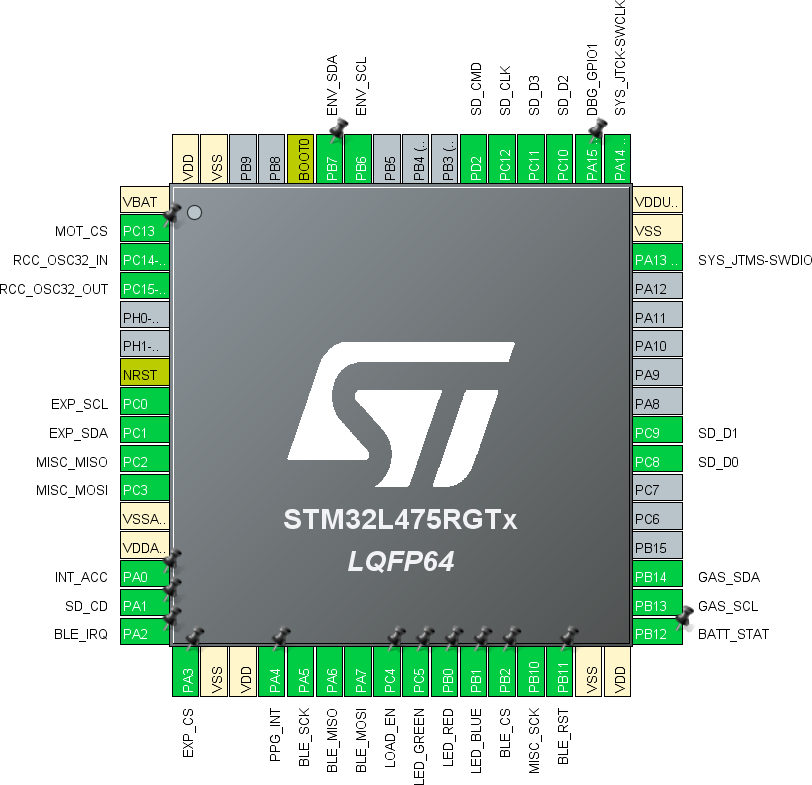
\includegraphics[width=.5\textwidth]{media/winter_cube.png}
	\end{frame}

	\begin{frame}
		\frametitle{Winter - State machine}
		\centering
		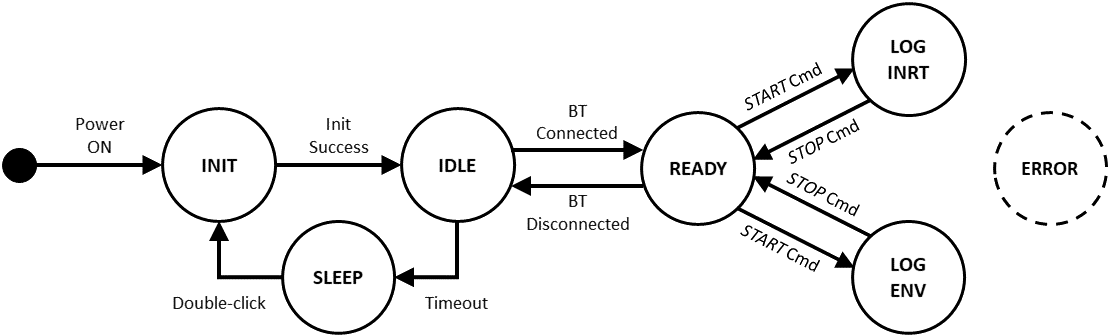
\includegraphics[width=.9\textwidth]{media/state_diagram.png}
	\end{frame}


	\begin{frame}
		\frametitle{Case study 2 - PPG}
		\textbf{Request:} develop a Winter expansion to perform a PPG measurement.\\
		\textbf{Additional constraints:}
		\begin{itemize}
			\item can be used as a probe for in-ear measurements;
			\item must be able to interface with the available Winter peripherals;
			\item on-board regulator for low-noise operation.
		\end{itemize}
	\end{frame}

	\begin{frame}
		\frametitle{PPG - Specification document}
		\only<1>{
			What should be in the specification document for the PPG expansion board?
			\begin{itemize}
				\item Sensor choices: \begin{itemize}
					\item Must have: pulse oximeter
					\item Maybe: axl
				\end{itemize}
				\item on-board regulator must be low noise (LDO)
				\item small form factor.
			\end{itemize}
		}
		\only<2>{
			Refining specifications:
			\begin{itemize}
				\item axl: small form factor, look for best performer afterwards;
				\item LDO: 1.8V regulator, small, look for lowest noise afterwards;
				\item tentative form factor of \SI{20}{\milli\meter}x\SI{8}{\milli\meter}.
			\end{itemize}
		}
	\end{frame}

	\begin{frame}
		\frametitle{PPG - Pulse oximetry sensor}
		The pulse oximetry sensor chosen is the \textbf{MAX30101}. Important features:
		\begin{itemize}
			\item \SI{5.6}{\milli\meter}x\SI{3.3}{\milli\meter}x\SI{1.55}{\milli\meter} package
			\item Integrated red, green and IR LEDs
			\item Ambient light filtering
			\item Good sigma-delta 18-bit ADC
			\item Selectable led driving current (\SI{0}{\milli\ampere}-\SI{50}{\milli\ampere})
		\end{itemize}
	\end{frame}

	\begin{frame}
		\frametitle{PPG - Accelerometer}
		\only<1>{
			Choices for PPG:
			\begin{itemize}
				\item same as Winter; must save space, board is small
				\item use $I^2C$, no need for high data rates, save 1 wire
				\item Important features:\begin{itemize}
					\item size first and foremost
					\item power consumption
					\item ODR
					\item noise
					\item full-scale
				\end{itemize}
			\end{itemize}
		}
		\only<2>{
			The \textbf{LIS2DH12} was chosen. Important features:
			\begin{itemize}
				\item \SI{2}{\milli\meter}x\SI{2}{\milli\meter}x\SI{1}{\milli\meter} package
				\item down to \SI{6}{\micro\ampere} current consumption @\SI{50}{\hertz} ODR
				\item $\pm 2$g - $\pm 16$g selectable full-scale;
				\item up to \SI{5}{\kilo\hertz} ODR (probably not needed)
				\item \SI{12}{\bit} resolution
			\end{itemize}
		}
	\end{frame}

	\begin{frame}
		\frametitle{PPG - LDO}
		The \textbf{ADP166} regulator with a fixed \SI{1.8}{\volt} output was chosen. Important features:
		\begin{itemize}
			\item low quiescent current \SI{\sim900}{\nano\ampere}
			\item \SI{72}{\decibel} PSRR @\SI{100}{\hertz}
			\item \SI{80}{\micro\volt} noise RMS
		\end{itemize}
	\end{frame}

	\begin{frame}
		\frametitle{PPG - Hardware rundown}
		We will see:
		\begin{itemize}
			\item PPG schematic
			\item PPG layout
		\end{itemize}
		After this, the final result will look something like this:
		\begin{center}
			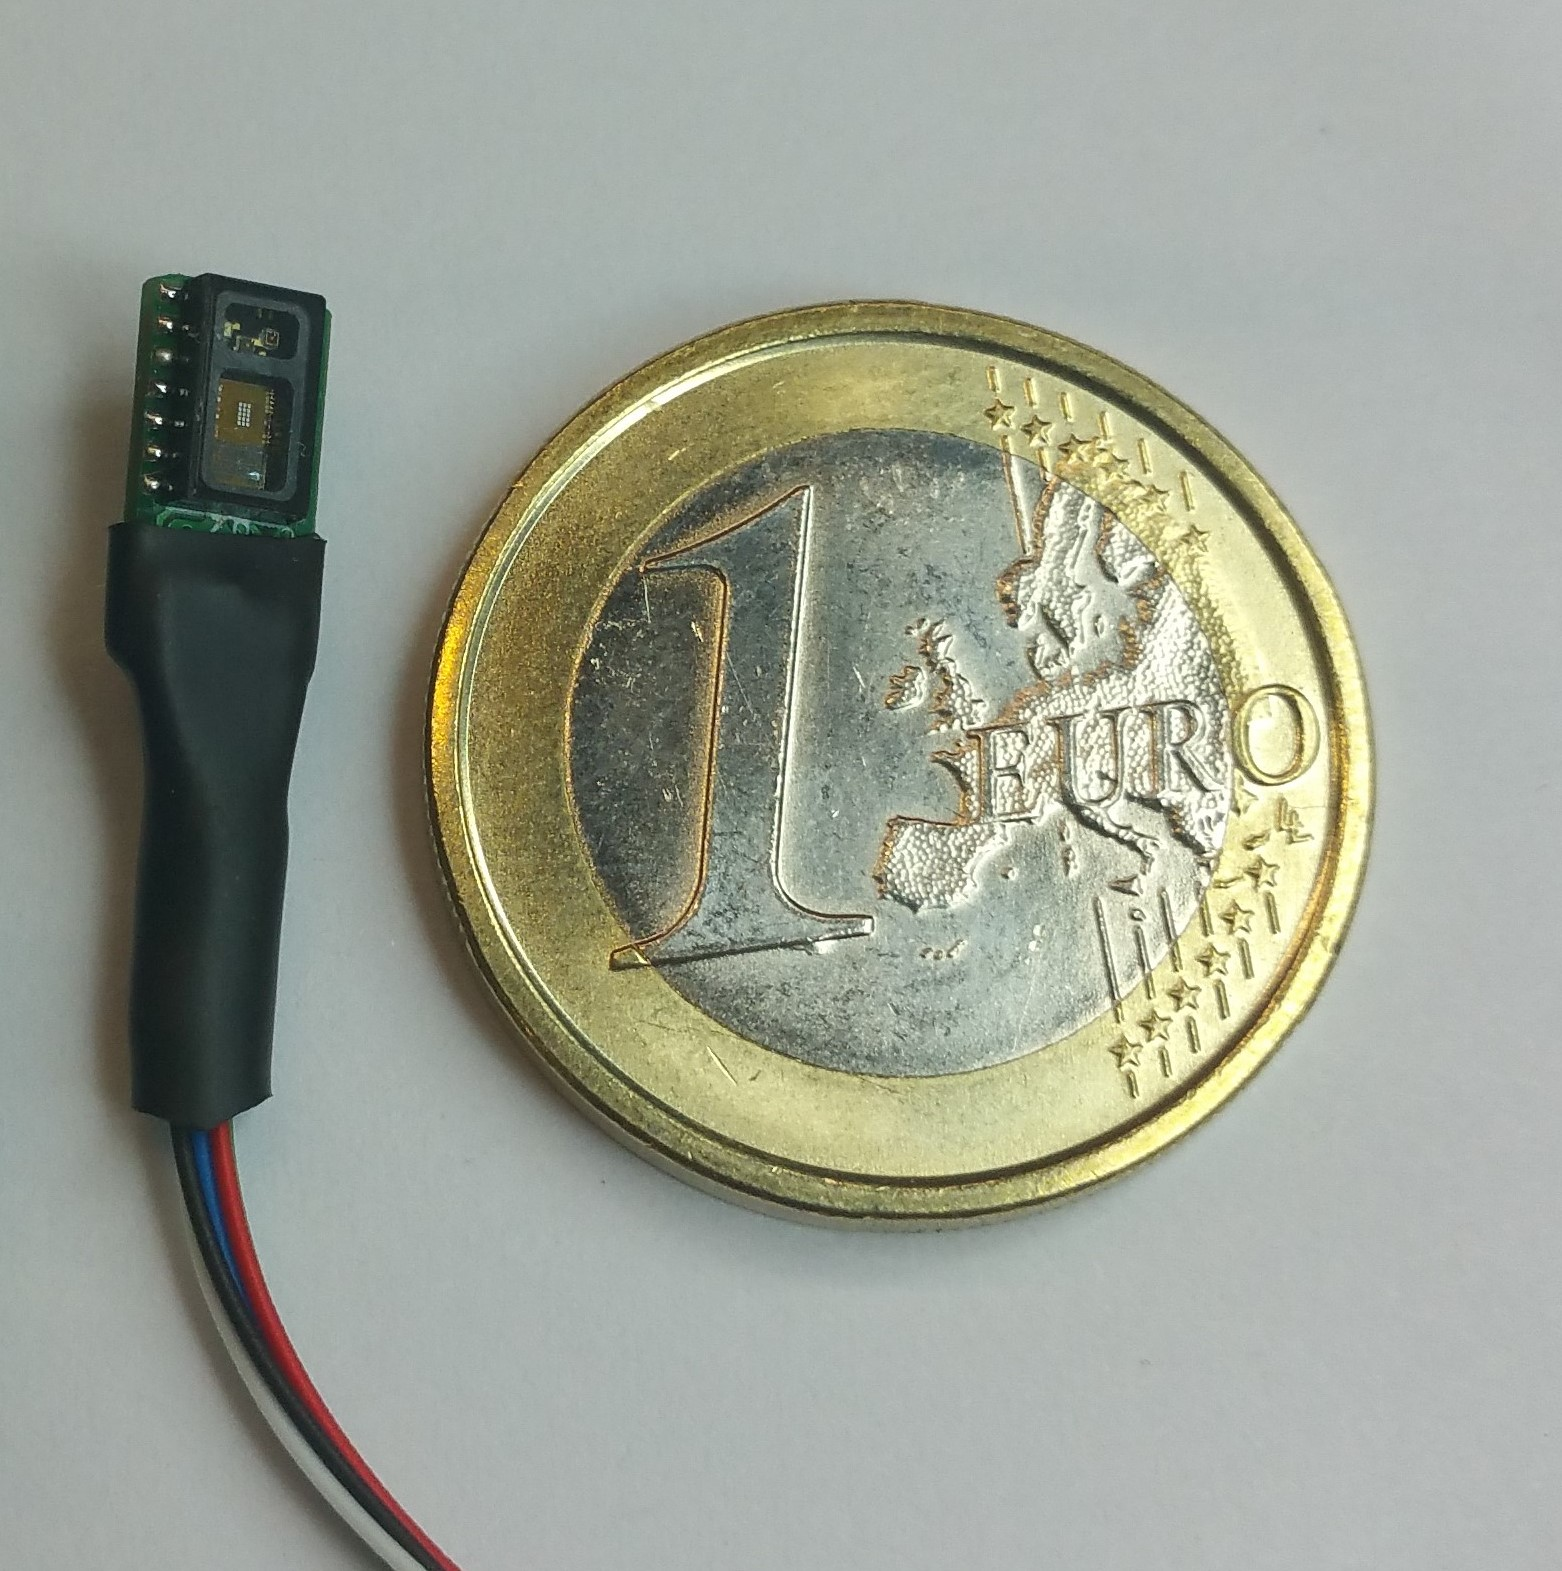
\includegraphics[width=.30\textwidth]{media/PPG.jpg}
		\end{center}
	\end{frame}

\end{document}
